\documentclass[11pt]{article}
\usepackage{amsmath,amssymb,amsthm}
\usepackage{graphicx}
\usepackage[margin=1in]{geometry}
\usepackage{fancyhdr}
\usepackage{amsmath}
\usepackage[utf8]{inputenc}
\setlength{\parindent}{0pt}
\setlength{\parskip}{5pt plus 1pt}
\setlength{\headheight}{13.6pt}
\graphicspath{parcial1src/}

\newcommand{\hmwkTitulo}{Tarea\ \#2}
\newcommand{\hmwkFechaEntrega}{01 de marzo de 2015}
\newcommand{\hmwkCurso}{Investigación de Operaciones}
\newcommand{\hmwkCursoSeccion}{Sección A}
\newcommand{\hmwkCursoInstructor}{Ing. Percy Barberena}
\newcommand{\hmwkNombreAutor}{Luis Carlos Contreras}
\newcommand{\hmwkAuthorID}{1990-11-3887}

\newcommand{\hmwkUniversidad}{Universidad Mariano Gálvez de Guatemala}
\newcommand{\hmwkFacultad}{Ingeniería en Sistemas de Información}
\newcommand{\hmwkSede}{Sede Chimaltenango}

\author{\textbf{\hmwkNombreAutor}\\ \textbf{ \vspace{0.1in}\hmwkAuthorID}}
\date{\hmwkFechaEntrega}

\pagestyle{fancy}
\lhead{\textbf{\hmwkNombreAutor}}
\chead{\textbf}
\rhead{\hmwkCurso}

\title{
	\textbf{\hmwkUniversidad} \\
	\hmwkFacultad \\
	\vspace{0.1in}\hmwkSede\\
    \vspace{2.5in}
    \textmd{\textbf{\hmwkTitulo}}\\
    \vspace{0.1in}\large{\hmwkCurso , \textit{\hmwkCursoInstructor }}
    \vspace{2.5in}
}

%Comandos para los problemas
\newcommand\problema[2]{\vspace{.01in}\textbf{#1: #2}\vspace{.5em}\hrule\vspace{.10in}}
\renewcommand\part[1]{\vspace{.10in}\textbf{(#1)}}
\newcommand\planteamiento{\vspace{.10in}\textbf{Planteamiento: }}
\newcommand\solucion{\vspace{.10in}\textbf{Solución: }}
\newcommand\conclusion{\vspace{.10in}\textbf{Conclusión: }}

\newcommand\obj{\vspace{.10in}\textit{Objetivo: }}
\newcommand\funcObj{\vspace{.10in}\textit{Función objetivo: }}

\begin{document}
\maketitle
\pagebreak

\problema{1}{Problema 1}

\planteamiento Una empresa dedicada a la venta de dos productos manufactureros, necesita saber cuántas unidades de cada producto debe producir para el próximo mes si el propósito consiste en maximizar los beneficios de los mismos. Los detalles de producción son los siguientes: Para producir una unidad del producto A, se necesitan dos horas de máquina y tres horas de mano de obra. Cada unidad del producto B necesita tres horas de tiempo de máquina y dos horas de tiempo de mano de obra. El tiempo semanal disponible de máquina es de 250 horas, mientras que de mano de obra se dispone de 180 horas semanales. Si la ganancia que se obtiene por cada producto A, es de Q.35.00 y por cada producto B, de Q.30.00; determine la utilidad máxima.

\solucion

\obj Maximizar los beneficios\\
\begin{tabular}{|c|c|c|c|}
\hline 
 & Producto A & Producto B &  \\ 
\hline 
Máquina & 2 & 3 & $\leq$ 250 \\ 
\hline 
Mano de obra & 3 & 2 & $\leq$ 180 \\ 
\hline 
\end{tabular}


\begin{table}[h]
\begin{tabular}{ll}
Función objetivo & $X_0=35A+30B$    \\
Sujeto a:        & $2A+3B \leq 250$ \\
                 & $3A+2B \leq 180$ \\
                 & $A,B \geq 0$    
\end{tabular}
\end{table}
Por lo tanto:
\begin{align*}
X_0-35A-30B &=0\\
2A+3B &=250\\
3A+2B &=180
\end{align*}

El resultado del sistema de ecuaciones es:
\begin{math}
\mathbf{\left(\begin{array}{rrr}X_0=2620&A=8&B=78\\\end{array}\right)}
\end{math}
\begin{center}
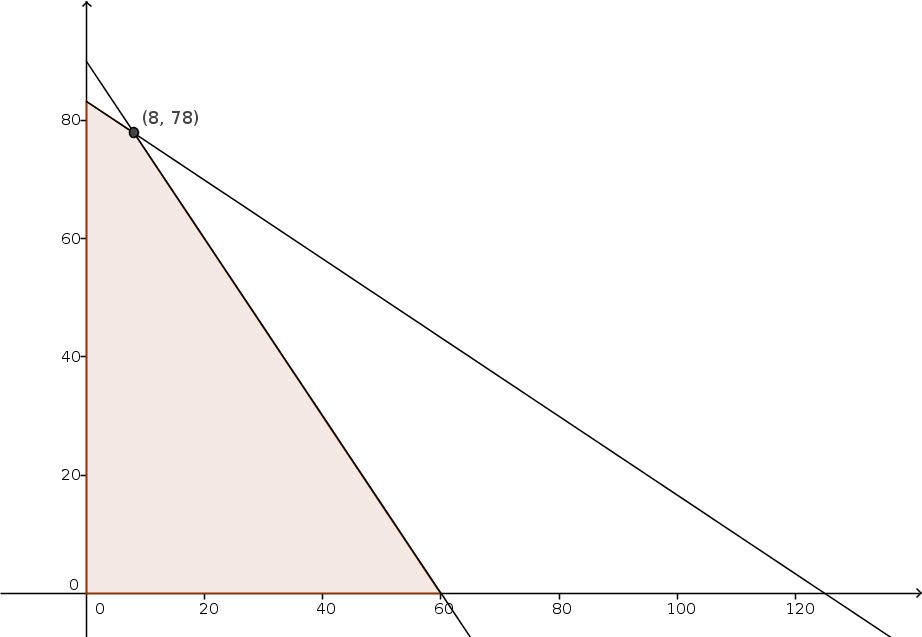
\includegraphics[scale=0.5]{parcial1src/problema1.png}
\end{center}
\conclusion Se deben producir 8 unidades del producto A y 78 unidades del pructo B para tener una ganancia máxima de Q.2620.00.

\pagebreak

\problema{3}{Ejercicio 3}
\planteamiento
Cierto fabricante produce sillas y mesas para las que requiere la utilización de dos secciones de producción, la sección de montaje y la de pintura. La producción de una silla requiere una hora de trabajo en la sección de montaje y de dos horas en la de pintura. Por su parte, la fabricación de una mesa precisa tres horas en la sección de montaje y de una hora en la de pintura. La sección de montaje sólo puede estar nueve horas diarias en funcionamiento, mientras que la de pintura sólo ocho horas. El beneficio produciendo mesas es el doble que el de sillas. ¿Cuál ha de ser la producción diaria de mesas y sillas para que el beneficio sea máximo?

\solucion

\obj Maximizar los beneficios

\begin{tabular}{c|c|c|c}
\hline 
 & Mesas & Sillas &  \\ 
\hline 
Montaje & 3 & 1 & $\leq$ 9 \\ 
\hline 
Pintura & 1 & 2 & $\leq$ 8 \\ 
\hline 
\end{tabular}

\begin{table}[h]
\begin{tabular}{ll}
Función objetivo & $X_0-2M-1S=0$    \\
Sujeto a:        & $3M+1S \leq 9$ \\
                 & $1M+2S \leq 8$ \\
                 & $M,S \geq 0$    
\end{tabular}
\end{table}

Por lo tanto:
\begin{align*}
X_0-2M-1S=0\\
3M+1S=9\\
1M+2S=8
\end{align*}

El resultado del sistema de ecuaciones es:
\begin{math}
\mathbf{\left(\begin{array}{rrr}X_0=7&M=2&S=3\\\end{array}\right)}
\end{math}

\begin{center}
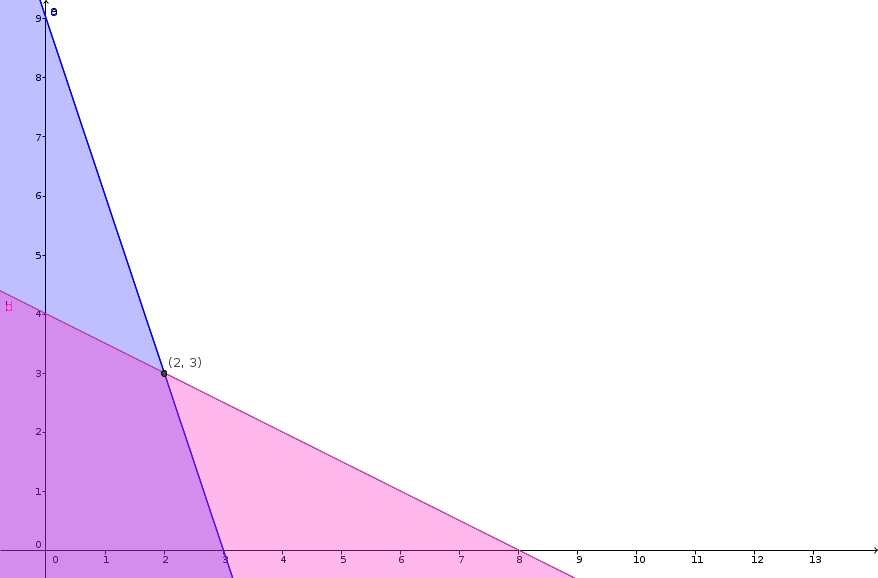
\includegraphics[scale=0.5]{parcial1src/problema3.png}
\end{center}
\conclusion Se deben producir 2 mesas M y 3 sillas S para obtener una ganancia de Q.7.00.
\pagebreak


\problema{5}{Ejercicio 5}
\planteamiento
Una empresa fabricante ingresó al negocio produciendo una calculadora de 12 funciones, la FC-12, que se vende a Q.6.00. Luego agregó una versión mejorada de 18 funciones, la FC-18, que se vende a Q.9.00. Los costos unitarios de producción son, para la FC.12 de Q.2.00 y para la FC18 de Q.3.00. La empresa puede fabricar cualquier combinación de calculadoras siempre y cuando no exceda su capacidad disponible. El tiempo de montaje de cada calculadora FC-12 es de 0.20 horas, y para la FC-28 es de 0.70 horas; disponiendo de 8,000 horas de trabajo en el mes. El departamento de mercadeo ha establecido que la empresa puede vender hasta 12,000 calculadoras en el mes sin importar la combinación en la cantidad de cada estilo de calculadora, pues ambas tienen aceptación en el mercado. Determine la cantidad de calculadoras de cada estilo que deben producirse a fin de maximizar la utilidad.

\solucion

\obj Maximizar la utilidad

\begin{tabular}{|c|c|c|c|}
\hline 
 & FC12 (A) & FC18 (B) &  \\ 
\hline 
Cantidad total & A & B & $\leq$ 12000 \\ 
\hline 
Horas de trabajo & 0.2 & 0.7 & $\leq$ 8000 \\ 
\hline 
\end{tabular}

\begin{table}[h]
\begin{tabular}{ll}
Función objetivo & $X_0 = 4A+6B$    \\
Sujeto a:        & $A+B \leq 12000$ \\
                 & $0.2A+0.7B \leq 8000$ \\
                 & $A,B \geq 0$    
\end{tabular}
\end{table}

Por lo tanto:
\begin{align*}
X_0-4A-6B &= 0\\
A+B &= 12000\\
0.2A+0.7B &= 8000
\end{align*}
El resultado del sistema de ecuaciones es:
\begin{math}
\mathbf{\left(\begin{array}{rrr}X_0=70400&A=800&B=11200\\\end{array}\right)}
\end{math}

\begin{center}
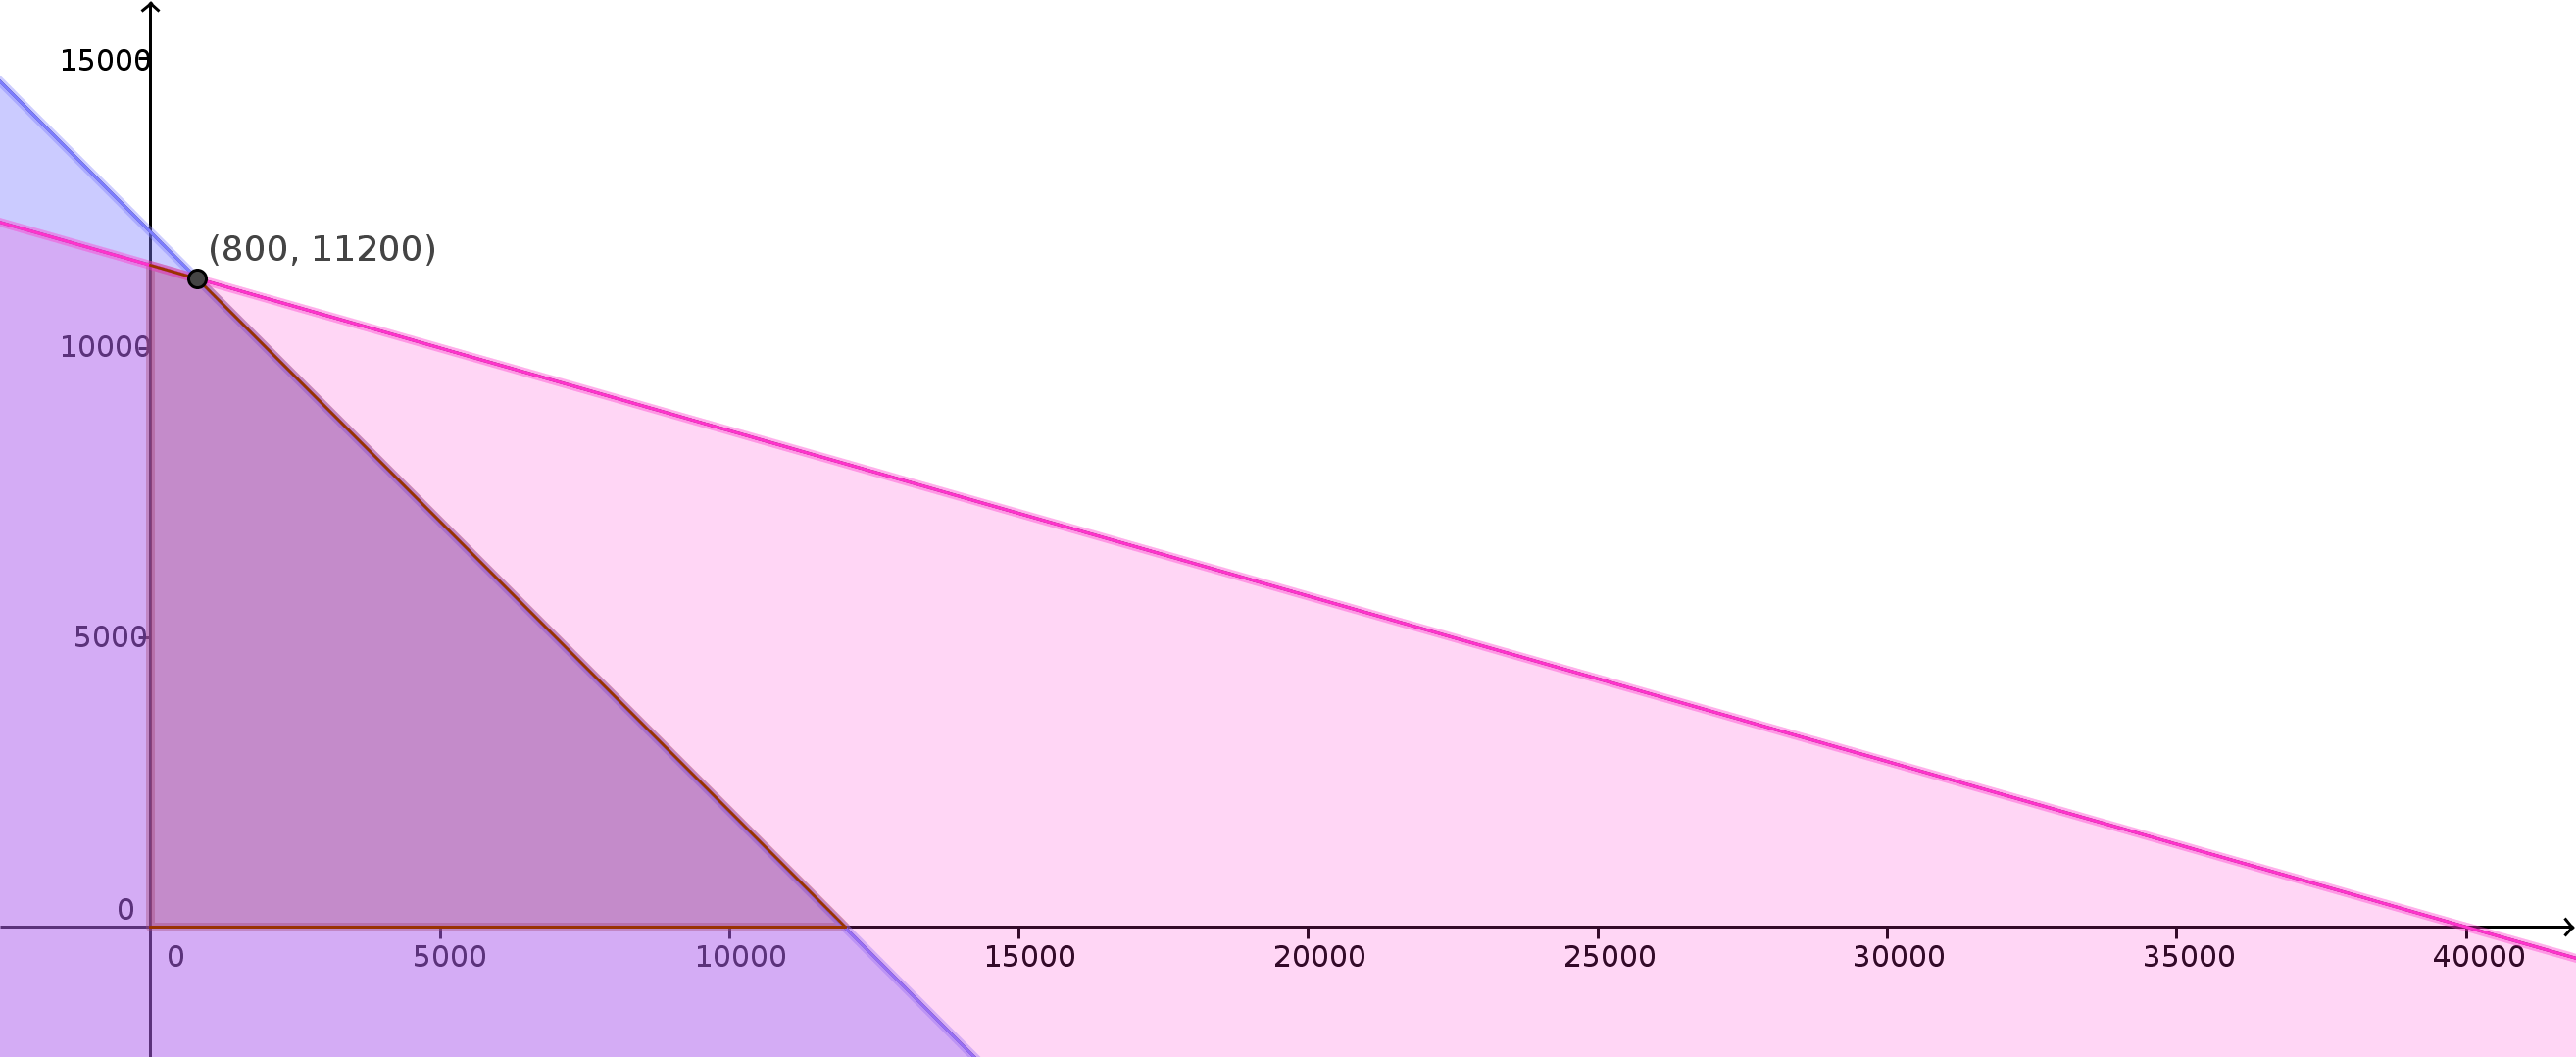
\includegraphics[scale=0.3]{parcial1src/problema5.png}
\end{center}
\conclusion Se deben producir 800 unidades de la FC12 y 11,200 de la FC18 para alcanzar la utilidad que serían Q.70,400.

\pagebreak

\problema{7}{Ejercicio 7}
\planteamiento
En una granja de crianza de cerdos y conejos, se dispone de un espacio para almacenanmiento de concentrado hasta 2,300 kilogramos. Si cada cerdo necesita 30 kilogramos de concentrado al mes y cada conejo 18 kilogramos; y se sabe que las horas de cuidados requeridos para un cerdo son 30 y para un conejo son 60, disponiendo de 3,500 horas presupuestadas al mes. Determine la cantidad de animales que deben criarse si la venta de cada uno representa un beneficio Q.525.00 por cabeza de cerdo y Q.375.00 por cabeza de conejo, de tal manera de maximizar la utilidad.

\solucion

\obj Maximizar la utilidad

\begin{tabular}{|c|c|c|c|}
\hline 
 & Cerdos (C) & Conejos (J) &  \\ 
\hline 
Concentrado & 30 Kg & 18 Kg & $\leq$ 2300 \\ 
\hline 
Horas de cuidado & 30 hr & 60 hr & $\leq$ 3500 \\ 
\hline 
\end{tabular}

\begin{table}[h]
\begin{tabular}{ll}
Función objetivo & $X_0 = 525C+375J$    \\
Sujeto a:        & $30C + 18J \leq 2300$ \\
                 & $30C + 60J \leq 3500$ \\
                 & $C,J \geq 0$    
\end{tabular}
\end{table}

Por lo tanto:
\begin{align*}
X_0 - 525C - 375J &= 0\\
30C + 18J &= 2300\\
30C + 60J &= 3500
\end{align*}
El resultado del sistema de ecuaciones es:
\begin{math}
\mathbf{\left(\begin{array}{rrr}X_0=41964.29&C=59.52&J=28.57\\\end{array}\right)}
\end{math}

\begin{center}
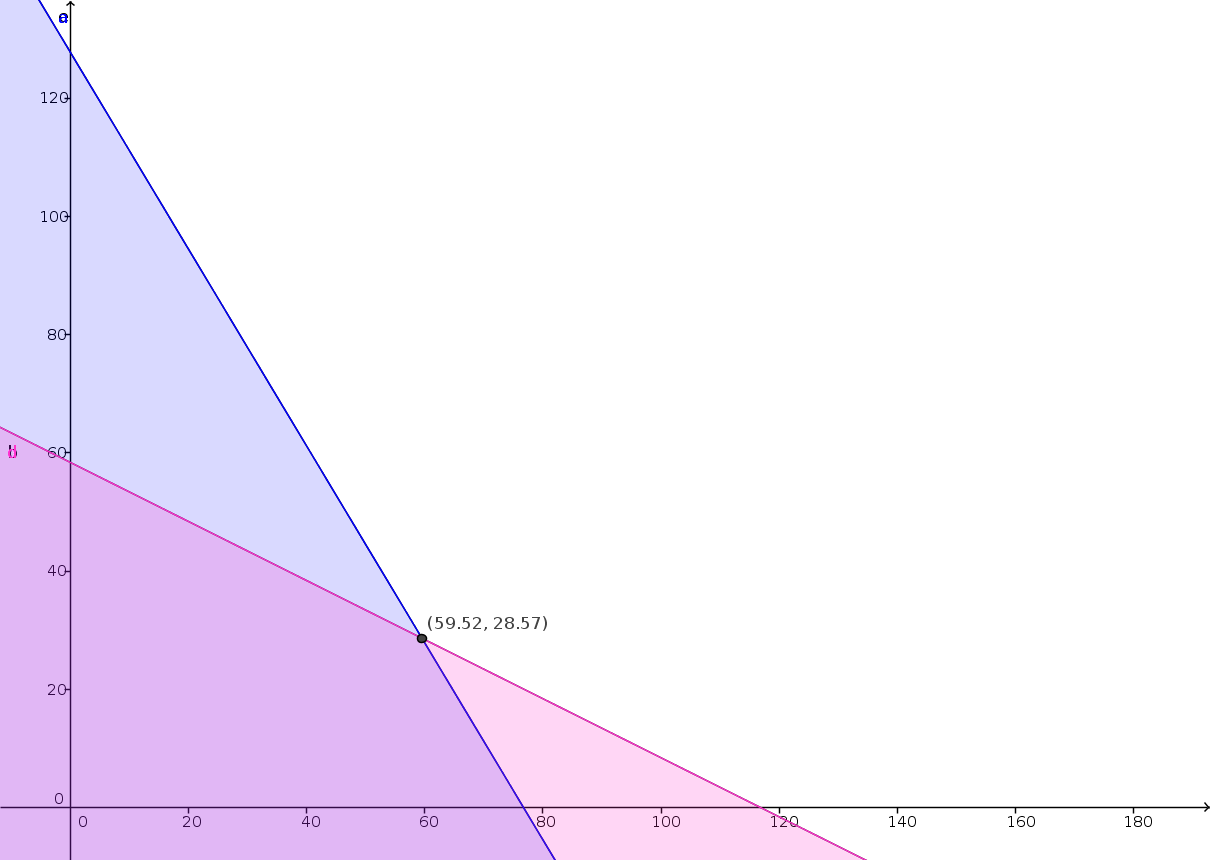
\includegraphics[scale=0.4]{parcial1src/problema7.png}
\end{center}
\conclusion Se deben criar 59 cerdos (59.52) y 28 conejos (28.57) para alcanzar una utilidad máxima de Q.41,964.29.

\pagebreak
\problema{9}{Ejercicio 9}
\planteamiento
Una conocida industria de calzado, lanza dos nuevos estilos en zapatos de seguridad industrial. El estilo R-metálico y el estilo R-seguridad. Se conoce que el estilo metálico aporta a las utilidades de la empresa Q.55.00 por unidad y que el estilo seguridad aporta Q.45.00 por unidad. El proceso general de la elaboración de los dos estilos conlleva tres fases dentro de la empresa; el departamento de troquelado, el de cosido y el de empaque. El estilo metálico requiere 0.30 horas en el primer departamento, 0.80 horas en el segundo y 0.50 horas en el tercero. El estilo seguridad requere 0.30 horas, 0.75 horas y 0.30 horas de producción en cada departamento, respectivamente. Las horas disponibles al mes son de 750 horas en troquelado, 1800 horas en cosido y 900 horas de empaque. Determine el volumen de producción óptimo de cada producto a fin de maximizar la utilidad total.


\obj Maximizar la utilidad

\begin{tabular}{|c|c|c|c|}
\hline 
 & R-Metálico (M) & R-Reguridad (D) &  \\ 
\hline 
Traquelado & 0.3 hrs & 0.3 hrs & $\leq$ 750 \\ 
\hline 
Cosido & 0.8 hr & 0.75 hr & $\leq$ 1800 \\ 
\hline 
Empaque & 0.5 hr & 0.3  hr & $\leq$ 900 \\ 
\hline 
\end{tabular}

\begin{table}[h]
\begin{tabular}{ll}
Función objetivo & $X_0 = 55M+45D$    \\
Sujeto a:        & $0.3M + 0.3D \leq 750$ \\
                 & $0.8M + 0.75D \leq 1800$ \\
                 & $0.5M + 0.3D \leq 900$ \\
                 & $M,D \geq 0$    
\end{tabular}
\end{table}

Por lo tanto:
\begin{align*}
X_0 - 55M - 45D &= 0\\
0.3M + 0.3D &= 750\\
0.8M + 0.75D &= 1800\\
0.5M + 0.3D &= 900
\end{align*}

El resultado de maximizar la función es:
\begin{math}
\mathbf{\left(\begin{array}{rrr}X_0=115000&M=1000&D=1333.33\\\end{array}\right)}
\end{math}

\conclusion Se deben producir 1,000 de tipo R-Metálico y 1,333 (1333.33) de tipo R-seguridad para alcanzar una utilidad máxima de Q.115,000.

\pagebreak
\problema{11}{Ejercicio 11}
\planteamiento
Una industria maquiladora dedicada a la confección de prendas de vestir para dama, se enfrenta al problema de maximizar la cantidad de docenas que puede producir de dos prendas líderes en el mercado en función de su capacdidad disponible. Las dos prendas son el "Panty estilo 3000" y el "Baby Doll, estilo 2025". En ambos casos, se utilizan para su confección las máquinas Zig-Zag y Overclock. Se tiene determinado el total de horas estándar a utilizar por cada docena producida, para cada máquina y estilo de la siguiente manera:

\begin{table}[h]
\begin{tabular}{|c|c|c|}
\hline
\textbf{Estilo prenda} & \textbf{Zig-Zag} & \textbf{Overclock} \\ \hline
3000                   & 0.185 hrs/doc    & 0.238 hrs/docs     \\ \hline
2025                   & 0.404            & 1.84 hrs/doc       \\ \hline
\end{tabular}
\end{table}

La jornada laboral es de 8 horas diarias y se cuenta con tres máquinas de overclock y tres máquinas de zig-zag para la confección de prendas, las cuales funcionan simultáneamente cada día para producir las cantidades necesarias.

\pagebreak
\problema{13}{Ejercicio 13}
\planteamiento
Recientemente el departamento de mercadotecnia de una empresa productora de artículos para el hogar determinó que los dos principales productos de la empresa por el volumen de ventas que normalmente generan, estaban decreciendo en sus aportes de beneficios financieros. Por lo tanto, se estableció que el volumen de ventas del producto 1 es cuando menos el 60\% de las ventas totales de los dos productos. Ambos productos utilizan la misma materia prima, cuya disponibilidad está limitada a 100 libras. Ambos productos I y II utilizan esta materia prima a razón de 2 lbs/unidad y 4 lbs/unidad, respectivamente. El precio de venta de los dos productos es de \$.20.00 y \$.40.00 por unidad. ¿Qué cantidad de cada producto debe promocionar y vender el departamento de mercadeo y ventas para maximizar la utilidad?


\obj Minimizar costo

\begin{tabular}{|c|c|c|c|}
\hline 
 & Maíz (M) & Harina de soya (H) &  \\ 
\hline 
Calcio & 0.01lb & 0.02lb & $\geq$ 1 \\ 
\hline 
Proteína & 0.9lb & 0.6lb & $\geq$ 60 \\ 
\hline 
Fibra & 0.2lb & 0.6lb & $\leq$ 40 \\ 
\hline 
\end{tabular}

\begin{table}[h]
\begin{tabular}{ll}
Función objetivo & $X_0 = 0.2M+0.6H$    \\
Sujeto a:        & $0.01M + 0.02H \geq 1$ \\
                 & $0.9M + 0.6H \geq 60$ \\
                 & $0.2M + 0.6H \leq 40$ \\
                 & $M,H \geq 0$    
\end{tabular}
\end{table}

Por lo tanto:
\begin{align*}
X_0 - 0.2M - 0.6H &= 0\\
0.01M + 0.02H &= 1\\
0.9M + 0.6H &= 60\\
0.2M + 0.6H &= 40
\end{align*}

El resultado de maximizar la función es:
\begin{math}
\mathbf{\left(\begin{array}{rrr}X_0=20&M=100&H=0\\\end{array}\right)}
\end{math}

\conclusion Se deben mezclar 20lb de maíz y 0lb de harina de soya para producir el alimento con menos costos de acuerdo a las restricciones. Esto generará un costo de Q.20.00.

\pagebreak
\problema{15}{Ejercicio 15}
\planteamiento
Un agricultor de un área rural, se dedica a la crianza de cerdos que consumen una mezvla especial de comida todos los días. El alimento puede prepararse con maíz y harina de soya de acuerdo a la siguiente descripción: Cada libra de maíz contiene: 0.01 lb. de calcio, 0.9 lb. de proteína y 0.2 lb de fibra. Cada libra de harina de soya contiene 0.02lb de calcio, 0.6 lb de proteína y 0.6lb de fibra. El costo por cada libra de maíz es de Q.0.20 y por cada libra de harina de soya es de Q.0.60. Los requsisitos diarios de alimentación de cada cerdo son: al menos 1\% de calcio, al menos 60\% de proteína y máximo 40\% de fibra. Determine la mezcla de alimentos por cada cerdo con el mínimo costo diario.

\solucion
\obj Minimizar costo

\begin{tabular}{|c|c|c|c|}
\hline 
 & Maíz (M) & Harina de soya (H) &  \\ 
\hline 
Calcio & 0.01lb & 0.02lb & $\geq$ 1 \\ 
\hline 
Proteína & 0.9lb & 0.6lb & $\geq$ 60 \\ 
\hline 
Fibra & 0.2lb & 0.6lb & $\leq$ 40 \\ 
\hline 
\end{tabular}

\begin{table}[h]
\begin{tabular}{ll}
Función objetivo & $X_0 = 0.2M+0.6H$    \\
Sujeto a:        & $0.01M + 0.02H \geq 1$ \\
                 & $0.9M + 0.6H \geq 60$ \\
                 & $0.2M + 0.6H \leq 40$ \\
                 & $M,H \geq 0$    
\end{tabular}
\end{table}

Por lo tanto:
\begin{align*}
X_0 - 0.2M - 0.6H &= 0\\
0.01M + 0.02H &= 1\\
0.9M + 0.6H &= 60\\
0.2M + 0.6H &= 40
\end{align*}

El resultado de maximizar la función es:
\begin{math}
\mathbf{\left(\begin{array}{rrr}X_0=20&M=100&H=0\\\end{array}\right)}
\end{math}

\conclusion Se deben mezclar 20lb de maíz y 0lb de harina de soya para producir el alimento con menos costos de acuerdo a las restricciones. Esto generará un costo de Q.20.00.


\pagebreak
\problema{17}{Ejercicio 17}
\planteamiento
El filete de lomo tiene un costo de \$12 por kilo y cada kilo contiene 83 calorías y 6 gramos de proteínas. El pollo rostizado tiene un costo de \$9 por kilo y cada kilo contiene 65 calorías y 2 gramos de proteínas. Con la información anterior, se desea realizazr una planeación dietética para una persona que debe consumir al menos 2,900 calorías y 190 gramos de proteínas. Determine la cantidad de filete de lomo y de pollo que debe consumir esta persona para cumplir con los requerimientos de dieta a un costo mínimo.

\obj Minimizar los costos

\begin{tabular}{|c|c|c|c|}
\hline 
 & Lomo (M) & Pollo (D) &  \\ 
\hline 
Calorías & 83  & 65 & $\geq$ 2900 \\ 
\hline 
Proteínas & 6 g & 2g & $\geq$ 190 \\ 
\hline 
\end{tabular}

\begin{table}[h]
\begin{tabular}{ll}
Función objetivo & $X_0 = 12L+9P$    \\
Sujeto a:        & $83L + 65P \geq 2900$ \\
                 & $6L + 2P \geq 190$ \\
                 & $L,P \geq 0$    
\end{tabular}
\end{table}

Por lo tanto:
\begin{align*}
X_0 - 12L - 9P &= 0\\
83L + 65P &= 2900\\
6L + 2P &= 190
\end{align*}

El resultado del sistema de ecuaciones es:
\begin{math}
\mathbf{\left(\begin{array}{rrr}X_0=416.38&L=29.241&P=7.27\\
\end{array}\right)}
\end{math}

\begin{center}
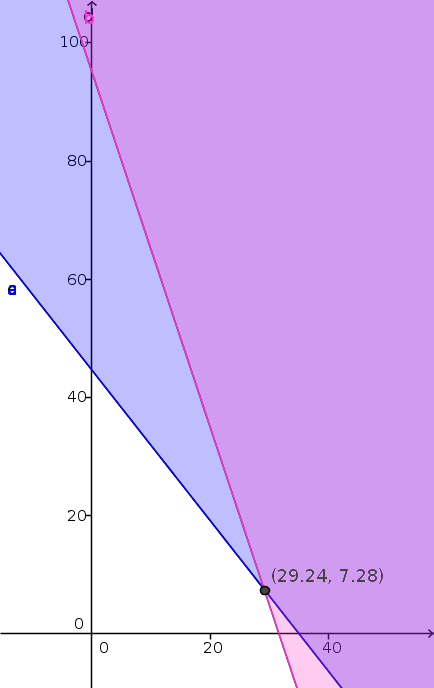
\includegraphics[scale=0.4]{parcial1src/problema17.png}
\end{center}

\conclusion Deben consumir 29.24 kilos de lomo y 7.27 kilos de filete de pollo; eso reducirá los costos a un mínimo de Q.416.38.
\end{document}
